\documentclass{article}
\usepackage[english]{babel}
\usepackage[letterpaper,top=2cm,bottom=2cm,left=2.5cm,right=2.5cm,marginparwidth=1.25cm]{geometry}

\usepackage{hyperref, booktabs, float}
\usepackage[leqno]{amsmath}
\usepackage{enumitem, nccmath,lipsum,amssymb,xcolor,xparse,listings, blindtext}
\usepackage[most]{tcolorbox}

\usepackage{graphicx}
\graphicspath{ {./attachments/} }

\NewDocumentCommand{\codeword}{v}{\texttt{\textcolor{blue}{#1}}}

\lstset{language=C, keywordstyle={\bfseries \color{blue}}}

\NewDocumentCommand{\mynote}{+O{}+m}{%
  \begingroup
  \tcbset{%
    noteshift/.store in=\mynote@shift,
    noteshift=1.5cm
  }
  \begin{tcolorbox}[nobeforeafter,
    enhanced,
    sharp corners,
    toprule=0.5pt,
    bottomrule=0.5pt,
    leftrule=0pt,
    rightrule=0pt,
    colback=green!10,
    #1,
    left skip=\mynote@shift,
    right skip=\mynote@shift,
    overlay={\node[right] (mynotenode) at ([xshift=-\mynote@shift]frame.west) {\textbf{Note:}} ;},
    ]
    #2
  \end{tcolorbox}
  \endgroup
  }
\makeatother

\newcommand{\mytext}[1]% #1 = same as intertext
{&\parbox{0.9\textwidth}{\rule{0pt}{.5\baselineskip}\\
\textrm{#1}\\
\rule{0pt}{.5\baselineskip}}&\\}

\newcounter{exercise}
\newcounter{problem}[exercise]
\newcommand{\myitem}{\stepcounter{problem}\tag*{\alph{problem})}}

\title{Lab 2: The filesystem, command line, and file manipulation}
\author{Mashenkov Timofei B23-CBS-02 \\ \href{mailto:t.mashenkov@innopolis.university}{t.mashenkov@innopolis.university}}
\begin{document}
\maketitle{}

\section{File system}

\subsection{How many inodes are in use on your system?}
\noindent

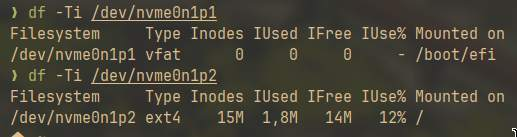
\includegraphics[width=320pt]{1_2.jpg}

12\% or 1,8M for main filesystem partition.

\subsection{What is the filesystem type of the EFI partition?}
\noindent

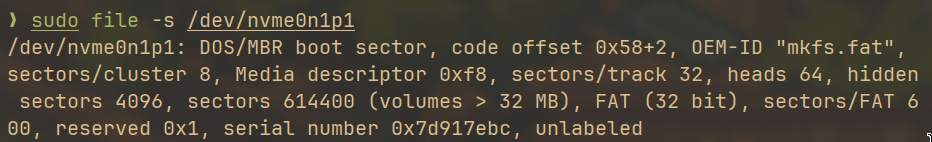
\includegraphics[width=320pt]{efi.jpg}

\codeword{FAT32} with \codeword{vfat} as mounting driver for Linux.

\subsection{What device is mounted at your root / directory? Show proof.}
\noindent

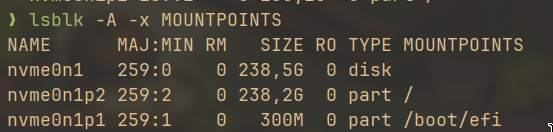
\includegraphics[width=320pt]{mount.jpg}

(Single/Main) SSD drive, second partition with filesystem.

\subsection{What is your partition UUID?}
\noindent

\begin{table}[H]
	\centering
	\begin{tabular}{|c|c|c|}
		\toprule
		name      & partition UUID                                & filesystem UUID               \\ \midrule
		nvme0n1p1 & b7ca2794-0cf1-4077-8861-3f62766f720d          & 7D91-7EBC                     \\
		nvme0n1p2 & \textbf{8a4f5599-5b48-4688-9b0c-90823630f73b} & b82d4971-7d9b-4214-9b96-d52b7 \\
		\bottomrule
	\end{tabular}
\end{table}

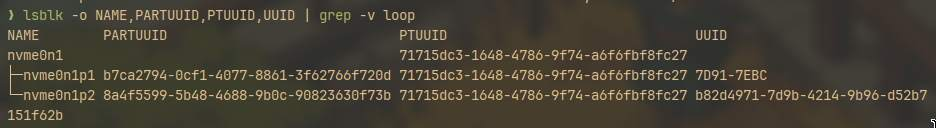
\includegraphics[width=320pt]{uuid.jpg}

\subsection{What is the function of /dev/zero?}
\noindent

This is special file, along with \codeword{/dev/null}, allows discarding data written to that file.
Unlike \codeword{/dev/null}, reads from this file always return bytes containing zero (\codeword{\0}) instead of EOF.

\section{Command line and file manipulation}

\subsection{Explain the role of the Pipe | in this command...}
\noindent

It redirects the stdout, which well contain the content of the file \codeword{/etc/apt/sources.list}, into the stdin of the command
\codeword{less}. \\

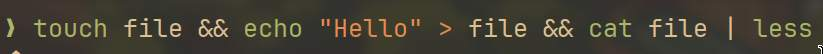
\includegraphics[width=320pt]{pipe.jpg}

Here, we create a file, after that echo some content inside, then concatenate it to stdout and redirect it to stdin of \codeword{less}.

\subsection{What does section 5 in man mean? And how can you find it?}
\noindent

According to \codeword{man man}, section 5 is for file formats and conventions.
To find out, if entity is in 5 section, we can use \codeword{man -k <command_name>}.

\subsection{What is the full file path of ls on your machine? How did you find it?}
\noindent

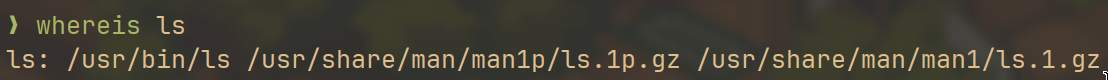
\includegraphics[width=320pt]{ls.jpg}

Here, we can see paths for the binary of \codeword{ls} and its man pages.

\subsection{Show two ways of renaming a file.}
\noindent

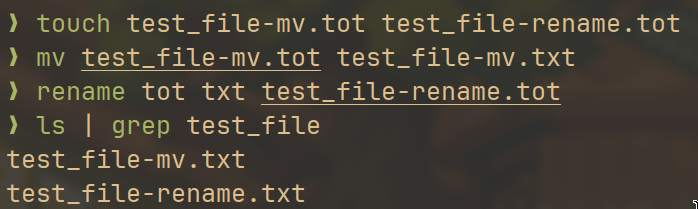
\includegraphics[width=320pt]{rename.jpg}

Also, we can use \codeword{cp} to copy file with new filename or extension and after that \codeword{rm} to remove old file.

\subsection{Create a compound command.}
\noindent

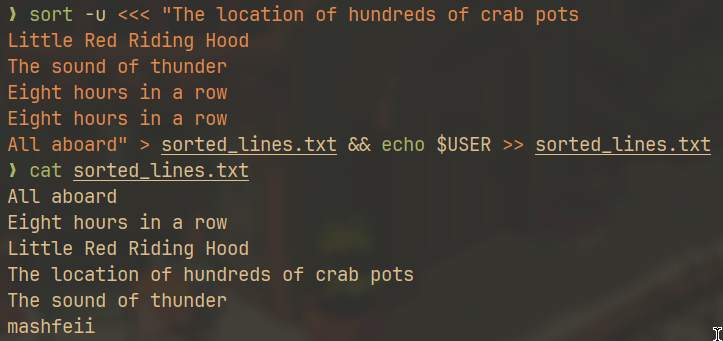
\includegraphics[width=320pt]{sort.jpg}

\subsection{What can you do to discard the output from the command ping 127.0.0.1?}
\noindent

\codeword{ping 127.0.0.1 &> /dev/null} or \codeword{ping 127.0.0.1 > /dev/null 2>&1}.\\

First variant redirects both stdout and stderr into the file, while in second case we redirect stderr into stdout, stdout into the file.
\codeword{/dev/null} is used to discard data, that we're trying to write into it, also, we could use \codeword{/dev/zero}.

\subsection{Show how you can sort input, append line numbers, and save the sorted result to a file.}
\noindent

The following siquence will read the multi-line input from console, until it gets EOF line, after we append line numbering for all lines
(here flag \codeword{b} specifies that we take \codeword{a} - all lines as our style variant),
finally we sort leaving the blank lines on their places and output to the file. \\

\codeword{cat << EOF | nl -ba | sort -s > filename.extension}

\subsection{Write out as much as possible ways to go from ... folder to ...}
\noindent

\begin{enumerate}
	\item \codeword{cd /home/$USER/testdir}
	\item \codeword{cd ../../home/$USER/testdir}
	\item \codeword{cd ~/testdir}
	\item \codeword{cd $HOME/testdir}
	\item \codeword{cd ~+/../../home/$USER/testdir}
	\item \codeword{~-/testdir} - in case you jupmed into \codeword{/usr/share} from home directory; as well as the \codeword{cd $OLDPWD/testdir}
	\item \codeword{$PWD/../../home/$USER/testdir}
\end{enumerate}

\subsection{Write a pipe...}
\noindent

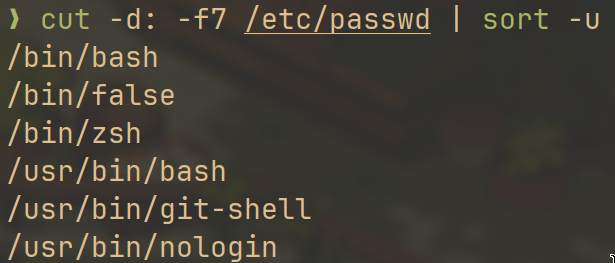
\includegraphics[width=320pt]{pipe-2.jpg}

Here, I cut each line of \codeword{/etc/passwd} using delimiter \codeword{:}, took 7th fragment and after that sort lines with \codeword{-u} flag to get unique lines.

\section{Bonus Questions}

\subsection{Find all man pages that contain word malloc. The result should be just a list of files}
\noindent

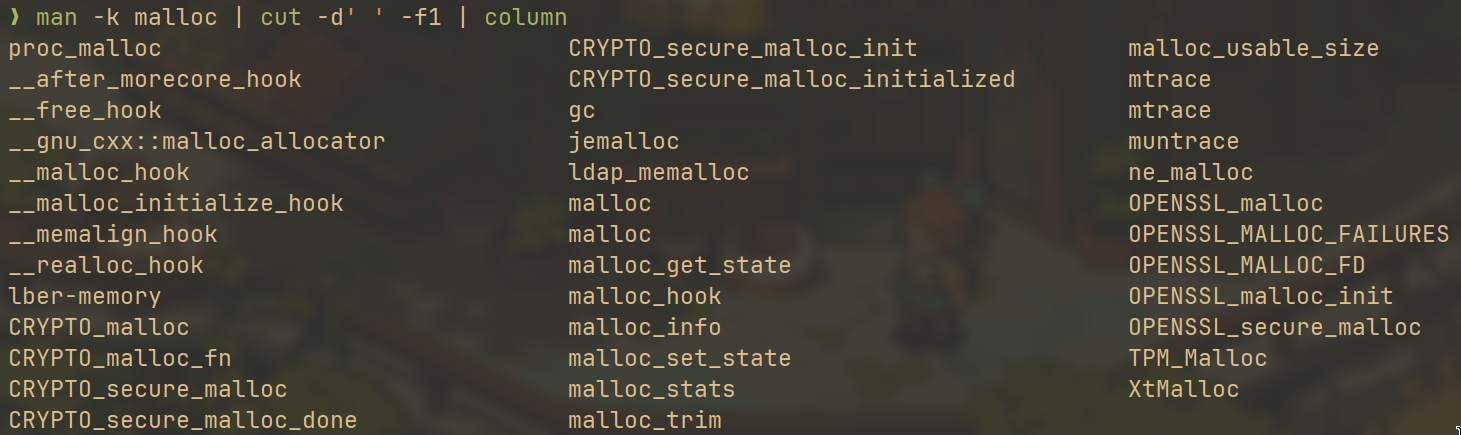
\includegraphics[width=480pt]{man.jpg}

\subsection{Write a one-liner...}
\noindent

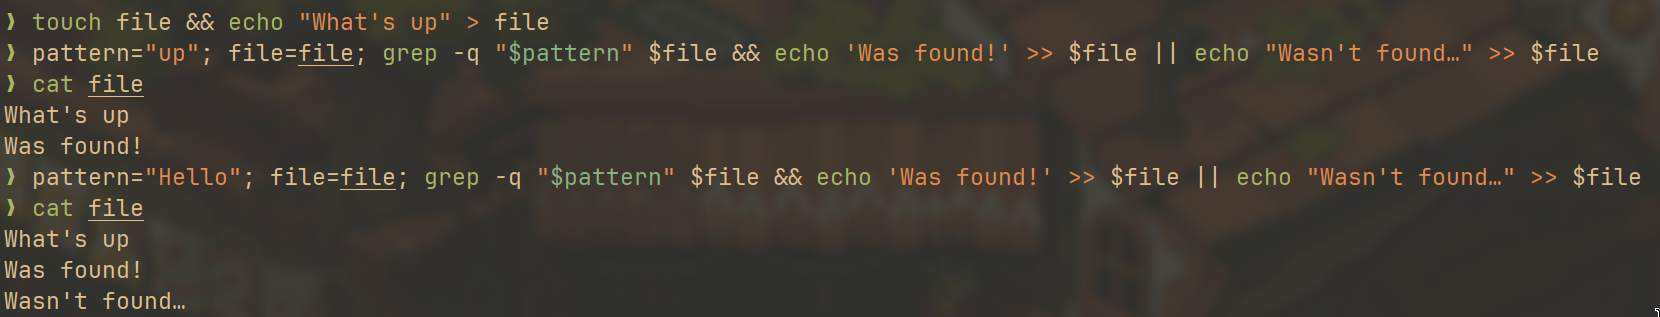
\includegraphics[width=480pt]{liner.jpg}

\end{document}
